\subsection{Phylogenetics and phylodynamics}

\subsubsection{Phylogenetic trees}

In evolutionary biology, a \defn{phylogeny}, or \defn{phylogenetic tree}, is a
graphical representation of the the evolutionary relationships among a group of
organisms or species (generally, \defn{taxa})~\autocite{haeckel1866generelle}.
The \defn{tips} of a phylogeny, that is, the nodes without any descendants,
correspond to \defn{extant}, or observed, taxa, while the \defn{internal nodes}
correspond to their common ancestors. The edges or \defn{branches} of the
phylogeny connect ancestors to their descendants. Phylogenies may have a
\defn{root}, which is a node with no descendants distinguished as the most
recent common ancestor of all the extant
taxa~\autocite{harding1971probabilities}. When such a root exists, the tree is
referred to as being \defn{rooted}; otherwise, it is \defn{unrooted}. The
structural arrangement of nodes and edges in the tree is referred to as its
\defn{topology}~\autocite{cavalli1967phylogenetic}. 

The branches of the tree may have associated lengths, representing either
evolutionary distance or calendar time between ancestors and their descendants.
The term ``evolutionary distance'' is used here imprecisely to mean any sort of
quantitative measure of evolution, such as the number of differences between
the DNA sequences of an ancestor its descendant, or the difference in average
body mass or height. This will be clarified below in
subsection~\ref{subsubsec:genetree}. A phylogeny with branch lengths in calendar
time units is often referred to as \defn{time-scaled}. In a time-scaled
phylogeny, the internal nodes can be mapped onto a timeline by using the tips
of the tree, which usually map to the present day, as a reference
point~\autocite{nee1992tempo}. The corresponding points on the timeline are
called \defn{branching times}, and the rate of their accumulation is referred
to as the \defn{branching rate}. Rooted trees whose tips are all the same
distance from the root are called \defn{ultrametric}
trees~\autocite{buneman1974note}. These concepts are illustrated in
Figure~\ref{fig:speciestree}.

\begin{figure}[ht]
  \centering
  \label{fig:speciestree}
  \includegraphics{speciestree}
  \caption[Illustration of a rooted, ultrametric, time-scaled phylogeny]
    {Illustration of a rooted, ultrametric, time-scaled phylogeny. The tips of
      the tree, which represent extant taxa, are placed at the present day on
      the time axis. Internal nodes, representing extinct common ancestors to
      the extant taxa, fall in the past. The topology of the tree indicates
      that cats and dogs are the most closely related pair of species, whereas
      fish is most distantly related to any other node in the tree.}
\end{figure}

\subsubsection{Species trees and transmission trees}
\label{subsubsec:speciestree}

A \defn{species tree} is a particular type of phylogeny in which the taxa are
species, and the branching times correspond to historical speciation events. In
general, we do not have access to the true tree relating a particular group of
extant species, as this would imply certain knowledge of speciation events in
the distant past. Therefore, all species trees considered by researchers are
estimates, based on the genetic or phenotypic similarity of the extant taxa,
the fossil record, or both. We discuss some of the challenges associated with
this estimation in subsection \ref{subsubsec:treeconv} below. However, for the
moment, we ignore these complications and consider what can be said about the
true species tree.

Speciation, which causes branching in a species tree, often occurs by an
\defn{allopatric} process, where a sub-population of organisms is isolated from
the original population by a geographic barrier~\autocite{coyne2004speciation}.
Over time, differing selection pressures on either side of the barrier, coupled
with genetic drift, cause the two populations to diverge genetically. This
eventually results in two distinct species, which will appear as two subtrees
or \defn{clades} in their species tree if descendants of both survive to the
present. Of course, this is not necessarily the case, as selection may cause
one or both of the new sub-populations or their descendants to become extinct.
On the other hand, selection may favour one of the sub-populations, allowing it
to expand into new regions or niches and possibly paving the way for subsequent
speciation events. Therefore, \comment{Is this a fair statement?} we can point
out two forces primarily responsible for the shapes of species trees:
geographic barriers, which cause branching, and selection, which controls which
lineages survive to the present and influences the branching rate.

A different type of tree used in the study of pathogens is a \defn{transmission
tree}. In such trees, tips represent infected hosts, while internal nodes
correspond to transmissions from one host to another. Transmission trees are
generally time-scaled \comment{Is this true?} and rooted, with the root
corresponding to the index case and branching times indicating times of
transmission. The internal nodes may be labeled with the donor of the
transmission pair, if this is known. The tips of the tree, rather than being
fixed at the present day, are placed at the time at which the individual was
discovered or their pathogen population sampled. Consequently, the transmission
tree may not be ultrametric, but may have tips located at varying distances
from the root. Such trees are said to have \defn{heterochronous} taxa or
samples~\autocite{drummond2003measurably}, in contrast to the
\defn{isochronous} samples found in macro-organisms species trees. A
transmission tree is illustrated in Figure~\ref{fig:contactnet} (right).

When considering epidemics of RNA viruses, transmission trees and species trees
are highly related. The viral population within a single host has often been
referred to as a \defn{quasispecies}~\autocite{domingo2012viral}, and due to
the fast evolutionary rate of these viruses, two hosts' viral populations are
invariably genetically distinct. The transmission process is functionally
identical to allopatric speciation, involving geographic isolation of a
sub-population in a new host and subsequent genetic divergence. However, for
the most part, it is not selection but rather host epidemiology which causes
certain lineages to proliferate while driving others to extinction. A host who
recovers, dies, or is isolated equates to an extinction in the transmission
tree. On the other hand, dense populations in frequent contact often experience
rapid epidemic growth, which causes similarly rapid accumulation of branching
points in the tree. 

The fact that these evolutionary (ie. speciation) and epidemiological processes
occur on the same time scale for RNA viruses~\autocite{drummond2003measurably}
is the basis for the field of
\defn{phylodynamics}~\autocite{grenfell2004unifying}. The similarity between
transmission and speciation means that it is possible to apply many of the
tools and techniques developed for species trees to viral transmission trees,
and interpret the results in the context of transmission rates and host
epidemiology. As a basic example, the lineages-through-time
plot~\autocite{nee1992tempo}, which plots the historical speciation rate
against time, can be used to quantify the incidence of new infections over the
course of an epidemic. \comment{Reference?} In
subsection~\ref{subsubsec:treeshape} below, we review some of these methods in
more detail, as well as several which have been developed specifically for
viral phylodynamics, and discuss what these methods can tell us about host
epidemiology.

Finally, we must note two important points. First, we have not yet considered
the selection pressures operating within a single host, such as immune
pressure, because these forces do not directly impact transmission trees unless
they cause a host to recover or die. Second, we reiterate that both
transmission trees and species trees are theoretical objects which are almost
never known with certainty for real data. Indeed, the estimation of
transmission trees is often problematic, and it is in such estimation that
within-host forces play a role. Both of these issues are discussed further
below in subsection~\ref{subsubsec:treeconv}, though we continue to ignore them
in the next subsection.

\subsubsection{Gene trees and viral phylogenies}
\label{subsubsec:genetree}

\subsubsection{Estimating transmission trees}
\label{subsubsec:treeconv}

Most applications of viral phylodynamics, including this project, aim to answer
epidemiological questions~\autocite{volz2013viral}. For example, phylodynamic
methods have been used to investigate the degree of
clustering~\autocite{hughes2009molecular} and the effect of elevated
transmission risk in acute infection~\autocite{volz2012simple} (a more thorough
review is given below in subsection~\ref{subsubsec:appphylo}). For these
applications, we are ultimately interested in the transmission tree, which is a
representation of an epidemiological process (transmission), as opposed to the
viral phylogeny, which represents a biological process (viral evolution). As
discussed above in subsection~\ref{subsubsec:speciestree}, transmission trees and
are in practice unknown, and must be estimated from available data. Here, we
review some of the ways to perform such estimation.

In principle, transmission trees can be reconstructed by on-the-ground
epidemiological methods, that is, by asking each person who they contacted.
This is particularly relevant for sexually transmitted diseases such as HIV,
where individuals are more likely to recall who they contacted and
when~\autocite{klovdahl1985social}. This kind of data is challenging to collect
in detail. Most commonly, when applying phylodynamics in practice, the
transmission tree is estimated from the viral
phylogeny~\autocite{volz2013viral}. As discussed above in
subsection~\ref{subsubsec:genetree}, the viral phylogeny is itself also estimated;
however, for the moment we ignore this complication and describe methods for
estimating the transmission tree if the viral phylogeny were known.

When we consider the fact that the viral phylogeny is not known with certainty,
the methods just described follow a two-step procedure. The first step is to
estimate the viral phylogeny, and the second step is to use it to estimate the
transmission tree.

\autocite{didelot2014bayesian} develop a Bayesian version of the two-step
approach. They first estimate a time-scaled phylogeny from viral samples, then
estimate the transmissions which took place along the phylogeny. Due to
within-host evolution, the transmissions are allowed to occur anywhere along
the branches, rather than being constrained to happen at branching points.
However, the authors admit that their method requires sampling of every
infected individual, although they indicate that it could be extended to relax
this assumption.

A different approach is undertaken by Jombart
\etal~\autocite{jombart2011reconstructing}, who build transmission trees
directly from sequence data without the intermediate step of constructing a
phylogeny. Their method finds the most likely geneology among the sampled
sequences, assuming that the that the common ancestors to sampled isolates are
themselves sampled. Although this may be a realistic assumption in the early
stages of an epidemic of a slower evolving pathogen, it is unlikely for
ancestors to be present among sequences sampled from an ongoing HIV epidemic
\comment{Needs a reference}.

Several alternative approaches have been developed which aim to
incorporate available epidemiological data as well. Cottam
\etal~\autocite{cottam2008integrating} first built a viral phylogeny, then
enumerated all transmission trees consistent with this phylogeny by labelling
the internal nodes of the phylogeny in every possible way. Each of the putative
transmission trees was assigned a likelihood based on infection time and
geographic separation. 


\subsubsection{Tree shapes}
\label{subsubsec:treeshape}

The aim of viral phylodynamics is to glean some kind of knowledge, about the
epidemic, the virus, or its hosts and their behaviour, by studying a phylogeny,
most often a transmission tree. Phylogenies are complex objects, and it is not
immediately obvious how to extract useful information from them with respect to
fitting a parameter. Standard statistical methods, built for numeric data
cannot be applied directly - for example, one cannot perform a regression of a
parameter of interest against a phylogeny. Therefore, before we discuss exactly
what phylodynamics can tell us about epidemics, and how it has been applied in
the past, we will review some of the methods for quantifying the shapes of
phylogenies and their similarity to each other.

\subsubsection{Applications of phylodynamics}
\label{subsubsec:appphylo}

\subsection{Contact networks}
\label{subsec:contactnet}

\subsubsection{Overview}

Epidemics spread through populations of hosts through \defn{contacts} between
those hosts. The definition of contact depends on the mode of transmission of
the pathogen in question. For an airborne pathogen like influenza, a contact
may be simple physical proximity, while for a sexually transmitted pathogen
like HIV, contacts would be sexual partnerships. A \defn{contact network} is a
graphical representation of a host population and the contacts among its
members. The \defn{nodes} in the network represent hosts, and \defn{edges}
represent contacts between them. 

Edges in a contact networks may be \defn{directed}, representing one-way
transmission risk, or \defn{undirected}, representing symmetric transmission
risk. For example, a network for an airborne epidemic would use undirected
edges, because the same physical proximity is required for a host to infect or
to become infected. However, a blood-borne infection spread through
transfusions would use undirected edges, since the donor has no chance of
transmitting to the recipient. Directed edges are also useful when the
transmission risk is not equal between the hosts, such as with HIV
transmission, where acting as the receptive partner carries a higher risk of
infection than acting as the insertive partner. In this case, a contact could
be represented by two directed edges, one in each direction between the two
hosts, with the edges annotated by what kind of risk they imply. In fact, it is
possible to represent an undirected edge by two symmetric directed edges. For
this reason, we consider only contact networks with directed edges in the
sequel. A directed contact network is shown in Figure \ref{fig:contactnet}
(left).

The path an epidemic takes through a contact network determines the topology of
the transmission tree relating the infected hosts. The initially infected node
who introduces the epidemic becomes the root of the tree. Each time a
transmission occurs, the lineage corresponding to the donor host in the tree
splits into two, representing the recipient lineage and the continuation of the
donor lineage. This correspondence is illustrated in figure
\ref{fig:contactnet}. It's important to note that, although the order and
timing of transmissions determines the tree topology uniquely, the converse
does not hold. That is, there are generally several orders of infection which
could lead to the same topology, since the labels on the internal nodes of the
tree are not available to the researcher.

\begin{figure}[ht]
  \centering
  \label{fig:contactnet}
  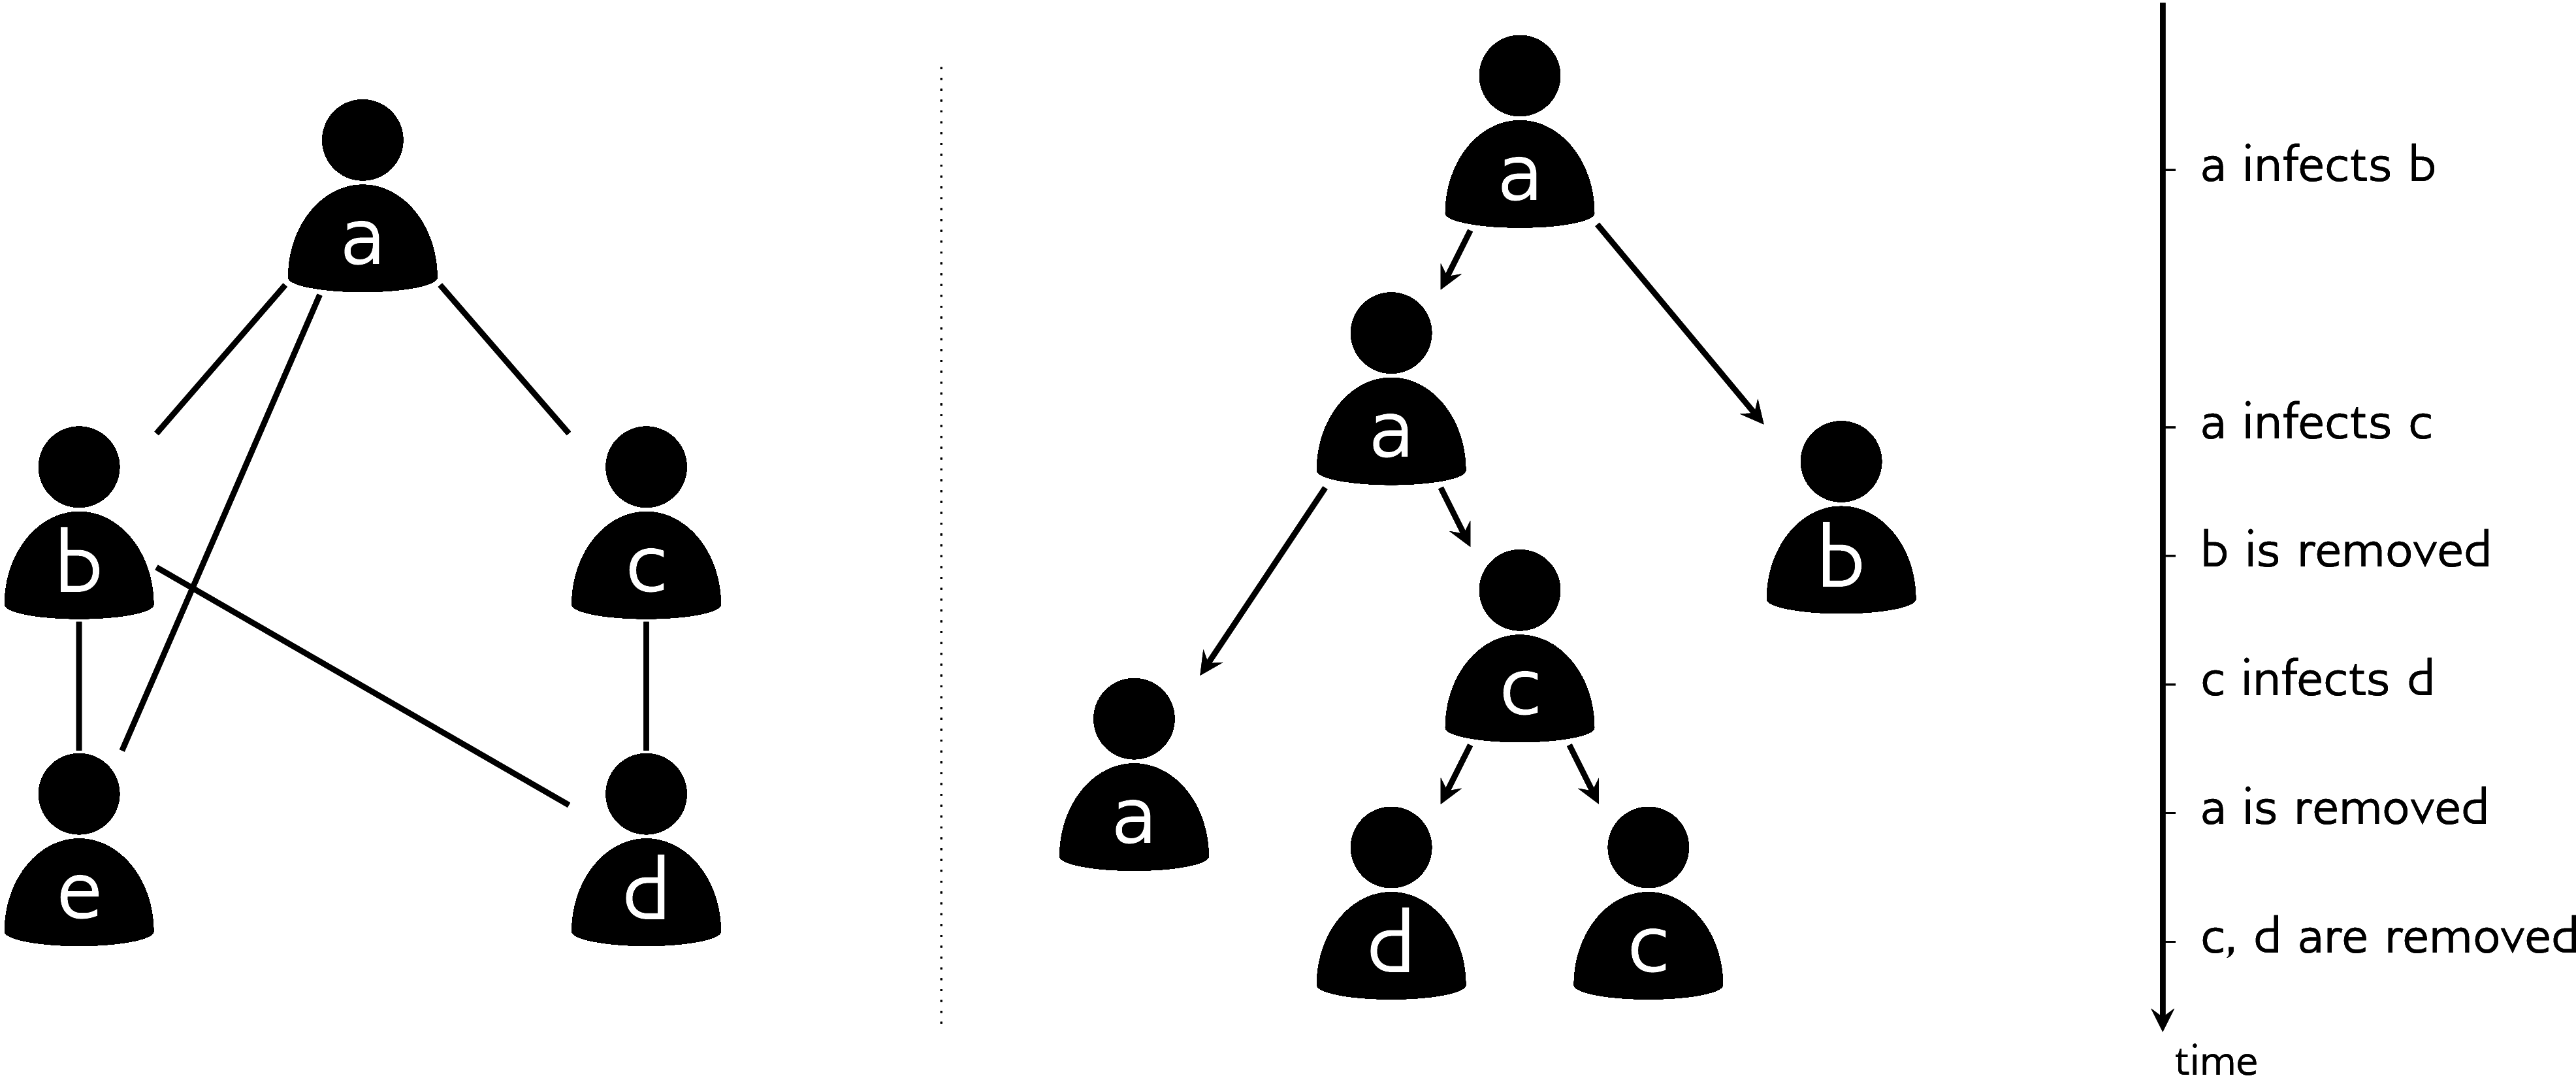
\includegraphics{contactnet}
  \caption[Illustration of a epidemic spread over a contact network]
  {Illustration of epidemic spread over a contact network. On the left, a
   contact network with five hosts, labelled A through E. Directed edges
   indicate six symmetric contacts among the hosts. Coloured, bolded edges
   represent transmissions. The epidemic began with node A, who transmitted to
   nodes B and C. Node C further transmitted to node D, and node E was not
   infected. On the right, the transmission tree topology corresponding to this
   scenario. Note that individual B was sampled before the other infected
   individuals, resulting in a tree with heterochronous tips.}
\end{figure}

\subsubsection{Generative models}
\label{subsubsec:generative}

%\subsection{Approximate Bayesian computation}

%Consider a model $M$, with parameters $\theta$, which we wish to fit to some
%observed data $D$. By ``fit'', we often mean that we want to find particular
%values $\hat{\theta}$ for the parameters which optimize the likelihood of our
%data given those parameters and the model,
%\[
%  \hat{\theta} = \argmax_\theta \Pr(D | M, \theta).
%\]
%This $\hat{\theta}$ is the \defn{maximum likelihood} parameter estimate. Note
%that we are employing a common abuse of notation here, where $\Pr(\cdots)$ is
%being unsed to refer to a probabilty \emph{density} rather than a true
%probability. Alternative to maximum likelihood, we may be interested less in a
%point estimate and more in the posterior distribution of possible values of
%$\theta$ given our data, $\Pr(\theta \mid M, D)$. This will be expanded upon
%below, but for the moment, for illustrative purposes, we restrict our attention
%to the maximum likelihood problem.
%
%If the model we are fitting is sufficiently simple, it may be possible to
%calculate $\hat{\theta}$ directly, using calculus. Most models do not admit
%analytic maximum likeilhood solutions, but if the likelihood any set of
%parameters can be calculated up to a normalizing constant, then
%${\Pr(D \mid M,\theta)}$ can be optimized numerically. A wide range of
%optimization strategies exist, the choice of which to use depending on the
%complexity of the model and whether or not we have access to the gradients of
%the likelihood function with respect to each of the parameters. The majority of
%modelling problems fit into this category, and numerical optimization is
%well-developed and extremely widely used.
%
%However, there are some cases, often when the observed data is of a complex
%type, that explicitly calculating the likelihood of some observed data is
%impossible, even up to a normalizing constant. For example, suppose that we
%want to model a chess player's behaviour. We will set up a simple one-parameter
%model which describes the chess playing process.  The parameter, $a \in [0, 1]$
%indicates the player's eagerness to remove his opponent's pieces from the
%board. We can write down an algorithm for the player's behaviour under such a
%model.
%
%% TODO: don't break this over the page
%
%\begin{algorithmic}
%  \While{the game is not over}
%    \If{I can capture an opponent's piece and $\Uniform(0, 1) < a$}
%      \State{capture the piece}
%    \Else
%      \State{make any other move at random}
%    \EndIf
%  \EndWhile
%\end{algorithmic}
%
%Suppose the observed data are the ending configurations of the board, after the
%player has concluded a game against an opponent with a known value of $a$. The
%model we have designed is very simple, but it is not obvious how to calculate
%the likelihood of a particular ending configuration. Indeed, it seems that the
%only way is to enumerate every possible path the game could have taken, and
%tabulate the ending configurations of each. Clearly, this is infeasible.
%Approximate Bayesian computation was designed for situations like these, where
%exact likelihoods are not available, perhaps due to the model involving an
%algorithm or generative process.

\subsection{Approximate Bayesian computation}
